\documentclass[xcolor=dvipsnames]{beamer}

\usepackage[T1]{fontenc}
\usepackage[utf8]{inputenc}
\usepackage[francais]{babel}
\usepackage{array}
\usepackage{tabularx}
\usepackage{multirow}
\usepackage{color}
\usepackage{colortbl}
\usepackage{textcomp}
\usepackage{xstring}
\usepackage{pifont}

%%% MACRO %%%


% FIXME Prendre en compte les majuscule déjà présente
\makeatletter
\@ifpackageloaded{xstring}{
	\newcommand\smallcaps[1]{\StrLeft{#1}{1}\scriptsize\uppercase{\StrGobbleLeft{#1}{1}}\normalsize }
}{
	\newcommand\smallcaps[1]{\textsc{#1}}
}
\makeatother



%===============================================================================
% Définit un type de puce pour une liste. Si le pakage "pifont" est chargé, il 
% est utilisé, sinon on met un tiret.
\makeatletter
\@ifpackageloaded{pifont}{
	\newcommand\goodItemArrow[0]{\ding{226}}
}{
	\newcommand\goodItemArrow[0]{-}
}
\makeatother



%===============================================================================
% Item de liste avec spécification de la puce et paramètre écrit en gras.
\newcommand\functionality[1]{
	\item[\goodItemArrow] \textbf{#1}\\
}



%===============================================================================
% Commande \Euro indépendante des paquets chargés 
\makeatletter
\@ifpackageloaded{eurosym}{
	\newcommand\Euro[0]{\euro{}}
}{
	\@ifpackageloaded{textcomp}{
		\newcommand\Euro[0]{\texteuro}
	}{
		\newcommand\Euro[0]{Euro}
	}
}
\makeatother



%===============================================================================
% Accès à des variables dans le document. 
%\makeatletter
%\let\titleName\@title
%\let\subtitleName\@subtitle
%\let\authorName\@author
%\makeatother



% Titre de la section courante (que dans beamer)
%\secname 
% Titre de la sous-section courante (que dans beamer)
%\subsecname





\title[Livraison - Bilan]{Surfaces de r\'evolution discrètes}
\subtitle{Livraison - Bilan}
\author[]{Zied \smallcaps{Ben} \smallcaps{Othmane} \\ Thomas \smallcaps{Benoist} \\ Adrien \smallcaps{Bisutti} \\ Lydie \smallcaps{Richaume}}
\institute{Universit\'e de Poitiers}
\date{2 mars 2016}

\usetheme{Madrid}
\usecolortheme{sidebartab}
\usefonttheme{professionalfonts}

\definecolor{fondtitre}{rgb}{0.0,0.35,0.7}
\setbeamercolor{palette primary}{bg=fondtitre}
\setbeamercolor{palette secondary}{bg=fondtitre!75!black}
\setbeamercolor{palette tertiary}{bg=fondtitre!55!black}
\setbeamercolor{palette quaternary}{bg=fondtitre!35!black}
\setbeamercolor{item}{fg=fondtitre}



%%% MACRO %%%


% Affichage du plan à chaque début de section
\AtBeginSection[]{
	\begin{frame}{Plan}
	  	\tableofcontents[currentsection, hideothersubsections]
	\end{frame}
}


% Nouvelle boîte pour le titre
\newenvironment<>{titleblock}[1]{%
	\setbeamercolor{block body}{fg=white, bg=fondtitre}%
	\begin{block}#2{#1}}{\end{block}}


% Vide la barre de navigation
\setbeamertemplate{navigation symbols}{}



%%% DOCUMENT %%%



\begin{document}


%===============================================================================
%	TITRE
%===============================================================================


\begin{frame}
	\titlepage
	
\includegraphics[width=2cm]{../Images/logo-Xlim.png}
	\hfill
	
\includegraphics[width=2cm]{../Images/logo_univ_poitiers.png}
\end{frame}



%===============================================================================
%	PLAN
%===============================================================================


\begin{frame}{Plan}
	\tableofcontents[hideallsubsections]
\end{frame}



%===============================================================================
%	INTRODUCTION
%===============================================================================

\section{Introduction}


% --- Contexte -----------------------------------------------------------------
	\begin{frame}{\secname}
		\begin{itemize}
			\item Nouvel algorithme conçu par \'Eric \smallcaps{Andres} et Ga\"elle \smallcaps{Largeteau}-\smallcaps{Skapin} pour mod\'eliser des surfaces de r\'evolution discrètes.
			\item Visualisation des r\'esultats avec Mathematica
		\end{itemize}
		\begin{figure}
			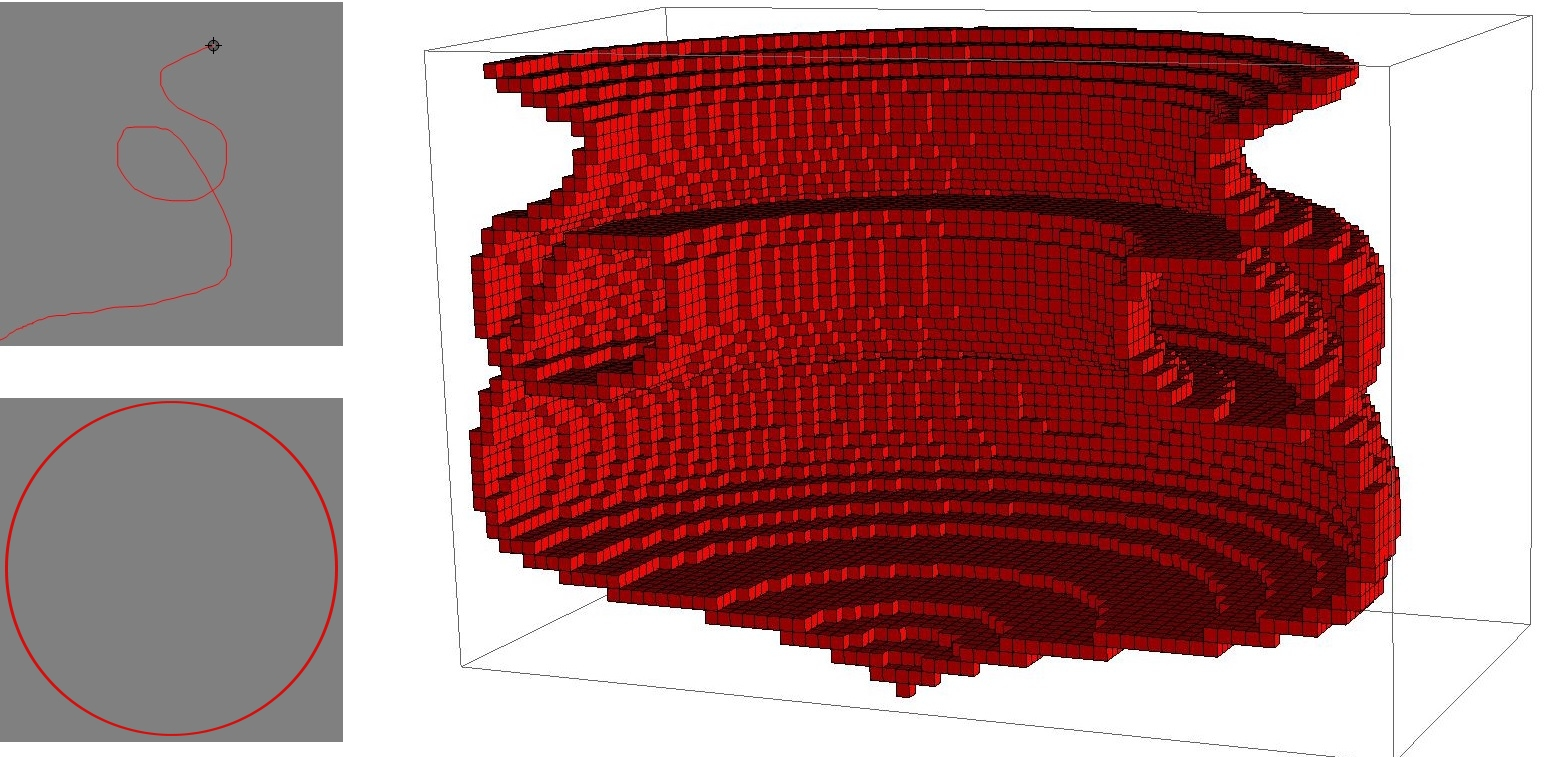
\includegraphics[height=3.8cm]{../Images/revolution2.jpg}
		\end{figure}
		\begin{itemize}
			\item Besoin d'un outil utilisable partout et par tous
		\end{itemize}
	\end{frame}
	
	

%===============================================================================
%	GESTION DU PROJET
%===============================================================================


\section{Planification}
	
	
	\subsection{Diagramme de Gantt}
	\begin{frame}{\subsecname}
		\begin{center}
			\href{run:ImagesLivraison/Gantt_ProjetDiscretReference.gif}{Diagramme pr\'evisionnel}\\
			\bigskip
			\href{run:ImagesLivraison/Gantt_ProjetDiscretRealise.gif}{Diagramme r\'ealis\'e}
		\end{center}
	\end{frame}
	
	
	\subsection{Livrables}
	\begin{frame}{\subsecname}
		\begin{center}
		\small
		{\renewcommand{\arraystretch}{1.3}
		\begin{tabular}{|c|>{\raggedright}m{4,5cm}|c|c|}
			\hline
			\textbf{\No} & \textbf{Livrable}
			& \textbf{Date pr\'evue} & \textbf{Date effective}\\
			\hline
			1 & R\'esultat de l'algorithme et interface & 23/12 
			& 18/01\\
			\hline
			2 & Application minimale & 21/01 & 25/01\\
			\hline
			2\textsuperscript{bis} & Multicoupe et param\`etres & --- & 29/01\\
			\hline
			3 & Courbes avec param\`etres modifiables et trac\'e \`a main
			lev\'ee & 29/01 & ---\\
			\hline
			4 & \'Equations et export & 19/02 & ---\\
			\hline
			5 & Application finale et documentation & 02/03 & ---\\
			\hline
		\end{tabular}}
		\end{center}
	\end{frame}



%===============================================================================
%	CAHIER DES CHARGES
%===============================================================================


\section{Fonctionnalités demandées}

% --- Surface ------------------------------------------------------------------
	\subsection{Génération des surfaces}
	\begin{frame}{\subsecname}
		\vspace{2cm}
	 	\begin{center}
		{\renewcommand{\arraystretch}{1.3}
		\begin{tabular}{|l|c|l}
			\cline{1-2}
			\textbf{Fonctionnalités} & \textbf{Niveau} &\\
			\cline{1-2}
			Génération de la surface & 1 & \Valid\\
			\cline{1-2}
			Diff\'erents algorithmes & 1 & \Valid\\
			\cline{1-2}
		\end{tabular}}
		\end{center}
		\vspace{3cm}
		\Valid~: R\'ealis\'e \hfill \NotCheck~: Non r\'ealis\'e
		\hfill \Modified~: Modifi\'e \hfill \Added~: Ajout\'e
	\end{frame}


% --- 2D -----------------------------------------------------------------------
	\subsection{Gestion des courbes}
	\begin{frame}{\subsecname}
		\vspace{1cm}
	 	\begin{center}
		{\renewcommand{\arraystretch}{1.3}
		\begin{tabular}{|l|c|l}
			\cline{1-2}
			\textbf{Fonctionnalités} & \textbf{Niveau} &\\
			\cline{1-2}
			Affichage des courbes & 1 & \Valid\\
			\cline{1-2}
			Mode de selection des courbes & 2 & \Valid\\
			\cline{1-2}
			Liste de courbes prédéfinies & 2 & \Valid\\
			\cline{1-2}
			Dessin de la m\'eridienne & 2 & \Valid\\
			\cline{1-2}
			Param\`etres des courbes & 2 & \Valid \Modified\\
			\cline{1-2}
			Afficher/cacher le rep\`ere des courbes & 4 & \NotCheck\\
			\cline{1-2}
			Entrer une \'equation & 5 & \Valid\\
			\cline{1-2}
		\end{tabular}}
		\end{center}
		\vspace{1cm}
		\Valid~: R\'ealis\'e \hfill \NotCheck~: Non r\'ealis\'e
		\hfill \Modified~: Modifi\'e \hfill \Added~: Ajout\'e
	\end{frame}


% --- 3D -----------------------------------------------------------------------
	\subsection{Manipulation de l'espace 3D}
	\begin{frame}{\subsecname}
	 	\begin{center}
		{\renewcommand{\arraystretch}{1.3}
		\begin{tabular}{|l|c|l}
			\cline{1-2}
			\textbf{Fonctionnalités} & \textbf{Niveau} &\\
			\cline{1-2}
			Choix des dimensions & 2 & \Valid \Modified\\
			\cline{1-2}
			Mouvement de cam\'era & 2 & \Valid\\
			\cline{1-2}
			Mise en \'evidence des courbes en 3D & 2 & \Valid\\
			\cline{1-2}
			Choix de la connexit\'e & 2 & \Valid \Modified\\
			\cline{1-2}
			Multi-coupes & 3 & \Valid\\
			\cline{1-2}
			Afficher/cacher limites espace 3D & 3 & \Valid \Modified\\
			\cline{1-2}
			Afficher/cacher rep\`ere 3D & 3 & \Valid\\
			\cline{1-2}
			Taille des voxels & 4 & \Valid \Modified\\
			\cline{1-2}
			Vue orthographique/perspective & 5 & \Valid\\
			\cline{1-2}
			Palette de couleur & -- & \Added\\
			\cline{1-2}
		\end{tabular}}
		\end{center}
		\Valid~: R\'ealis\'e \hfill \NotCheck~: Non r\'ealis\'e
		\hfill \Modified~: Modifi\'e \hfill \Added~: Ajout\'e
	\end{frame}


% --- Export -------------------------------------------------------------------
	\subsection{Export et sauvegarde}
	\begin{frame}{\subsecname}
		\vspace{1.5cm}
	 	\begin{center}
		{\renewcommand{\arraystretch}{1.3}
		\begin{tabular}{|l|c|l}
			\cline{1-2}
			\textbf{Fonctionnalités} & \textbf{Niveau} &\\
			\cline{1-2}
			Export 3D & 3 & \Valid\\
			\cline{1-2}
			Export impression 3D & 3 & \Valid\\
			\cline{1-2}
			Export PNG & 4 & \Valid\\
			\cline{1-2}
			Sauvegarde des courbes & 5 & \Valid \Modified\\
			\cline{1-2}
			Chargement des courbes & 5 & \Valid \Modified\\
			\cline{1-2}
		\end{tabular}}
		\end{center}
		\vspace{2cm}
		\Valid~: R\'ealis\'e \hfill \NotCheck~: Non r\'ealis\'e
		\hfill \Modified~: Modifi\'e \hfill \Added~: Ajout\'e
	\end{frame}


% --- Autre --------------------------------------------------------------------
	\subsection{Autre}
	\begin{frame}{\subsecname}
		\vspace{2cm}
	 	\begin{center}
		{\renewcommand{\arraystretch}{1.3}
		\begin{tabular}{|l|c|l}
			\cline{1-2}
			\textbf{Fonctionnalités} & \textbf{Niveau} &\\
			\cline{1-2}
			Aide utilisateur & 3 & \Valid \Modified\\
			\cline{1-2}
			Choix de la langue & 5 & \Valid\\
			\cline{1-2}
			Ajout courbes personnalisées & 5 & \NotCheck\\
			\cline{1-2}
		\end{tabular}}
		\end{center}
		\vspace{2.5cm}
		\Valid~: R\'ealis\'e \hfill \NotCheck~: Non r\'ealis\'e
		\hfill \Modified~: Modifi\'e \hfill \Added~: Ajout\'e
	\end{frame}



%===============================================================================
%	CONCLUSION
%===============================================================================


\section{Conclusion}


% --- Rappel -------------------------------------------------------------------
\begin{frame}{\secname}
	\begin{itemize}
		\item Documentation technique non livr\'e
		\item Projet extensible, code réutilisable
	\end{itemize}
\end{frame}


% --- Remerciment --------------------------------------------------------------
\begin{frame}{}
	\bigskip
	\bigskip
	\begin{titleblock}{}
		\begin{center}
			\smallskip
			\Large Surfaces de r\'evolution discrètes\\
			\medskip
			\small Livraison - Bilan
			\smallskip
		\end{center}
	\end{titleblock}

	\bigskip
	\begin{center}
		Merci de votre attention.\\
		\medskip
		Avez-vous des questions\,?			
	\end{center}

	\bigskip
	\bigskip
	
\includegraphics[width=2cm]{../Images/logo-Xlim.png}
	\hfill
	
\includegraphics[width=2cm]{../Images/logo_univ_poitiers.png}
\end{frame}


\end{document}


